\documentclass[12pt,oneside]{article}
\usepackage{makeidx,anysize,mflogo,xspace,float,epsfig,url}
\usepackage{amsmath,amsfonts,amssymb,a4wide} 
\usepackage[utf8]{inputenc}
%\usepackage[francais]{babel}
%\usepackage[french]{babel}
\urlstyle{sf}
%\usepackage{subcaption}
\usepackage[colorlinks = true,
linkcolor = blue,
urlcolor  = blue,
citecolor = blue,
anchorcolor = blue]{hyperref}
\usepackage{graphicx}
\usepackage{graphics}
\usepackage{float}
\usepackage[toc,page]{appendix} 
\usepackage{caption}
\usepackage{colordvi} %??
\usepackage{listings} 
\usepackage{subfigure}
\usepackage{subfloat}
\usepackage[dvipsnames]{xcolor}
\usepackage{multicol}
\usepackage{tikz}
\usepackage{array}
\usepackage{comment}
\graphicspath{{./figures/}}
%\usepackage[labelsep=quad,indention=10pt]{subfig}
\definecolor{grey}{rgb}{0.95,0.95,0.95} % on définit la couleur grise
	% (c'est un gris très clair)
	\definecolor{red}{rgb}{1.0,0.0,0.0} 
	\definecolor{green}{rgb}{0.0,1.0,0.0}
	\definecolor{blue}{rgb}{0.0,0.0,1.0}
	\lstloadlanguages{Python,bash,Java,C,C++,csh,make,sh}%%[Visual]Basic,xml}
	\lstset{frame=none,basicstyle=\footnotesize,breaklines,tabsize=2,captionpos=b,
		prebreak={\hbox{$\rightarrow$}},postbreak={\hbox{$\hookrightarrow$}},
		showstringspaces=false,backgroundcolor=\color{grey}\bfseries,
		keywordstyle=\color{blue},commentstyle=\color{PineGreen}\textit,
		stringstyle=\color{red}\ttfamily,abovecaptionskip=2pt,aboveskip=0pt,
		belowskip=0pt,belowcaptionskip=0pt,numbers=none,columns=fullflexible, backgroundcolor=\color{grey}}
%left,numberstyle=\footnotesize,
%		stepnumber=2,numbersep=1pt}

\begin{document}


\begin{center}
{\bf \Large Base designs} \\ \ \\
S. Denis, B. Maréchal G. Goavec-M\'erou, J.-M Friedt \\ \ \\ \today
\end{center}

This document aims at making a breve description of basic RF functions that can be set-up, using Vivado and the fpga\_ip repository. It assumes acquired the a priori knowledge on the OscillatorIMP ecosystem, otherwise refer to : \href{[https://github.com/oscimp/oscimpDigital]}{https://github.com/oscimp/oscimpDigital}.
The points discussed, listed below, are wrapped up in the example of a control loop design, with modulation and demodulation. A summary table of the IP blocks that can be used to build a numerical RF setup is given in the next pages. 

\begin{multicols}{2}
\begin{enumerate}
\setlength\itemsep{-0.1cm}
\item Reminder on signal dynamics
\item Webserver
\item Double voltage source
\item Double DDS
\item Amplitude modulation V1
\item Amplitude modulation V2
\item Frequency and phase modulation of a NCO
\item Demodulation
\item Filtering
\item Monitoring
\item Example to a control loop
\item FAQ
\end{enumerate}
\end{multicols}


\section{Reminder on signal dynamics}

Regardless of the presented functions, it's obviously better to optimize the dynamic of a signal to the range of data available. This first minimizes the part of noise of the electronics with respect to the signal. Secondly if the signal dynamic exceeds the range available, there is an overflow. For instance $14~bits$ signed data represent a range of $\pm 13~bits$ ie. from $-8192$ to $8191$ samples. Above $8191$ samples, there is an overflow and the signal returns to the beginning of the range, ie. $-8192$. Representation in Fig.\ref{fig:overflow}.

\begin{figure}[h!tb]
\begin{center}
\includegraphics[width=0.5\linewidth]{figures/overflow.jpg}
\caption{Overflow on the top and bottom of a sine.}
\label{fig:overflow}
\end{center}
\end{figure}

\newpage 
\vspace*{-1.5cm}
\hspace*{-1cm}
\begin{tabular}{|>{\centering\arraybackslash}m{.3\linewidth} | >{\centering\arraybackslash}m{.3\linewidth} |>{\centering\arraybackslash}m{.3\linewidth}|}
\hline
  & & \\
\textbf{IP} & \textbf{Equivalent RF function {\color{BlueViolet}or numeric function}} &\textbf{ Equivalent scheme with {\color{OliveGreen} tuneable entries}} \\
 & & \\

\hline
\includegraphics[width=5cm,trim={1cm 9cm 1cm 8cm},clip]{figures/Offset.pdf} &Tuneable amplitude offset, bias.&
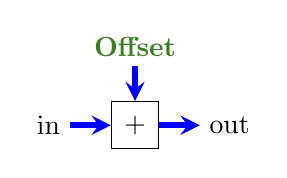
\begin{tikzpicture}
\node[draw, rectangle, minimum size=.6cm] (plus) {$+$};
\node[xshift=-1.1cm] (i) {in};
\node[yshift=+1cm] (c) {\textbf{{\color{OliveGreen}Offset}}};
\node[xshift=+1.2cm] (o) {out};
\draw [->,>=stealth,line width=2pt,blue] (i) -- (plus);
\draw [->,>=stealth,line width=2pt,blue] (plus) -- (o);
\draw [->,>=stealth,line width=2pt,blue] (c) -- (plus);
\end{tikzpicture}  \\

\hline
\includegraphics[width=4.8cm,trim={1cm 9.5cm 1cm 9cm},clip]{figures/splitter.pdf} &Splitter&
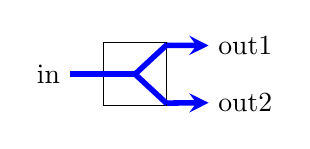
\begin{tikzpicture}
\node[draw, rectangle, minimum size=.8cm] (spl) {};
\node[xshift=-1.1cm] (i) {in};
\node[xshift=+1.4cm,yshift=+0.36cm] (o1) {out1};
\node[xshift=+1.4cm,yshift=-0.36cm] (o2) {out2};
\draw [-,line width=2pt,blue] (spl.west) -- (spl.center);
\draw [-,line width=2pt,blue] (spl.center) -- ([yshift=-0.03cm] spl.north east);
\draw [-,line width=2pt,blue] (spl.center) -- ([yshift=+0.03cm] spl.south east);
\draw [->,>=stealth,line width=2pt,blue] ([yshift=-0.04cm] spl.north east) -- (o1);
\draw [->,>=stealth,line width=2pt,blue] ([yshift=+0.04cm] spl.south east) -- (o2);
\draw [-,>=stealth,line width=2pt,blue] (i) -- (spl);
\end{tikzpicture}   \\

\hline
\includegraphics[width=6cm,trim={6.2cm 11.5cm 4cm 11.5cm},clip]{figures/addsub.pdf} &\hspace*{0.8cm}Combiner.\newline {\color{BlueViolet} Add or subtract signals.}& 
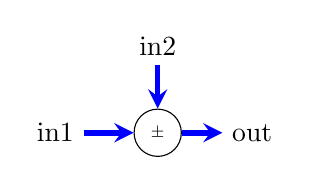
\begin{tikzpicture}
\node[draw, circle, minimum size=.6cm] (plus) {\tiny $\pm$};
\node[xshift=-1.3cm] (i) {in1};
\node[yshift=+1.1cm] (c) {in2};
\node[xshift=+1.2cm] (o) {out};
\draw [->,>=stealth,line width=2pt,blue] (i) -- (plus);
\draw [->,>=stealth,line width=2pt,blue] (plus) -- (o);
\draw [->,>=stealth,line width=2pt,blue] (c) -- (plus);
\end{tikzpicture}  \\

\hline
\includegraphics[width=4.6cm,trim={1cm 9.5cm 1cm 8.5cm},clip]{figures/mixer.pdf} &Mixer& 
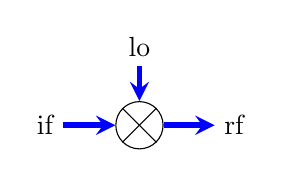
\begin{tikzpicture}
\node [circle, draw ,minimum size=.6cm] (mix) {};
\draw [-] (mix.south west) -- (mix.north east);
\draw [-] (mix.south east) -- (mix.north west);
\node [xshift=-1.2cm] (l) {if};
\node [yshift=+1cm] (u) {lo};
\node [xshift=+1.2cm] (r) {rf};
\draw [->,>=stealth,line width=2pt,blue] (l) -- (mix);
\draw [->,>=stealth,line width=2pt,blue] (u) -- (mix);
\draw [->,>=stealth,line width=2pt,blue] (mix) -- (r);
\end{tikzpicture}  \\

\hline
\includegraphics[width=4.8cm,trim={1cm 9cm 1cm 8cm},clip]{figures/fir.pdf} &\hspace*{0.6cm}Tuneable filter.\newline {\color{BlueViolet}FIR with decimation option.}& 
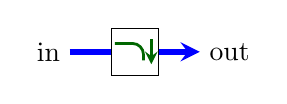
\begin{tikzpicture}
\node[draw, rectangle, minimum size=.6cm] (fir) {};
\node[xshift=-1.1cm] (i) {in};
\node[xshift=+1.2cm] (o) {out};
\draw [-, line width=1pt, color=black!60!green, rounded corners] ([xshift=.05cm,yshift=-.2cm] fir.north west) -| ([xshift=-.2cm,yshift=+.2cm] fir.south east);
\draw [->,>=stealth, line width=1pt, color=black!60!green] ([xshift=-.1cm,yshift=-.15cm] fir.north east) -- ([xshift=-.1cm,yshift=+.15cm] fir.south east);
\draw [line width=2pt,blue] (i) -- (fir);
\draw [->,>=stealth,line width=2pt,blue] (fir) -- (o);
\end{tikzpicture}  \\

\hline
\includegraphics[width=4.5cm,trim={1cm 10cm 1cm 9.5cm},clip]{figures/exp.pdf}\newline
\includegraphics[width=5cm,trim={2cm 11cm 2cm 10.5cm},clip]{figures/shift1.pdf} & {\footnotesize Can be assimilated to $2^m$ amplifiers or attenuators.\newline
{\color{BlueViolet}Are used to adapt the data size between blocks, or to select the range of the numeric signal.\newline
Expander: crop end of world, expand beginning of word. Shift: crop beginning of world, expand end of word.}}& 
\hspace*{0.45cm}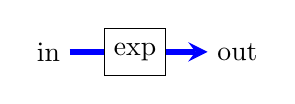
\begin{tikzpicture}
\node[draw, rectangle, minimum size=.6cm] (exp) {exp};
\node[xshift=-1.1cm] (i) {in};
\node[xshift=+1.3cm] (o) {out};
\draw [line width=2pt,blue] (i) -- (exp);
\draw [->,>=stealth,line width=2pt,blue] (exp) -- (o);
\end{tikzpicture} \newline
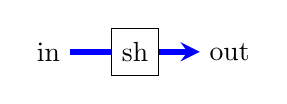
\begin{tikzpicture}
\node[draw, rectangle, minimum size=.6cm] (exp) {sh};
\node[xshift=-1.1cm] (i) {in};
\node[xshift=+1.2cm] (o) {out};
\draw [line width=2pt,blue] (i) -- (exp);
\draw [->,>=stealth,line width=2pt,blue] (exp) -- (o);
\end{tikzpicture} 
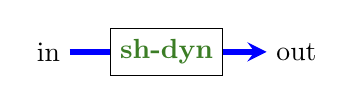
\begin{tikzpicture}
\node[draw, rectangle, minimum size=.6cm] (exp) {\textbf{{\color{OliveGreen}sh-dyn}}};
\node[xshift=-1.5cm] (i) {in};
\node[xshift=+1.65cm] (o) {out};
\draw [line width=2pt,blue] (i) -- (exp);
\draw [->,>=stealth,line width=2pt,blue] (exp) -- (o);
\end{tikzpicture}  \\

\hline

\includegraphics[width=4cm,trim={7.5cm 13.4cm 12.3cm 13.2cm},clip]{figures/switch.pdf} &Switch& 
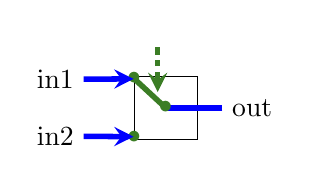
\begin{tikzpicture}	
\usetikzlibrary{arrows}
\node[draw, rectangle, minimum size=.8cm] (spl) {};
\node[xshift=+1.1cm] (i) {out};
\node[yshift=+0.9cm,xshift=-0.1cm] (s) {};
\node[xshift=-1.4cm,yshift=+0.36cm] (o1) {in1};
\node[xshift=-1.4cm,yshift=-0.36cm] (o2) {in2};
\node[OliveGreen, yshift=+0.37cm, xshift=-0.4cm]{$\bullet$};
\node[OliveGreen, yshift=-0.37cm, xshift=-0.4cm]{$\bullet$};
\draw [-,line width=2pt,blue] (spl.east) -- (spl.center);
\draw [-, line width=2pt,OliveGreen] (spl.center) -- ([yshift=-0.03cm] spl.north west);
\draw [<-,>=stealth,line width=2pt,blue] ([yshift=-0.04cm] spl.north west) -- (o1);
\draw [<-,>=stealth,line width=2pt,blue] ([yshift=+0.04cm] spl.south west) -- (o2);
\draw [<-,>=stealth,line width=2pt,OliveGreen,dash dot] ([yshift=+0.2cm,xshift=-0.1cm] spl.center) -- (s);
\draw [-,line width=2pt,blue] (i) -- (spl);
\node[OliveGreen]{$\bullet$};
\end{tikzpicture} \\

\hline

\end{tabular}

\newpage
\vspace*{-1.5cm}
\hspace*{-1cm}
\begin{tabular}{|>{\centering\arraybackslash}m{.3\linewidth} | >{\centering\arraybackslash}m{.3\linewidth} |>{\centering\arraybackslash}m{.3\linewidth}|}
\hline
  & & \\
\textbf{IP} & \textbf{Equivalent RF function {\color{BlueViolet}or numeric function}}&\textbf{ Equivalent scheme with {\color{OliveGreen}tuneable entries}} \\
 & & \\
 
 \hline
 \includegraphics[width=4.2cm,trim={2cm 10.5cm 2cm 10cm},clip]{figures/mean.pdf} &\hspace*{0.45cm}Moving average.\newline
 {\color{BlueViolet}Decimation of $2^n$ with averaging: slows the data flow.}
 &
 \begin{tikzpicture}
 \node[draw, rectangle, minimum size=.6cm] (exp) {$\sum~2^n$};
 \draw [->,>=stealth, line width=1pt] ([xshift=-.3cm,yshift=-.15cm] fir.north east) -- ([xshift=-.3cm,yshift=+.15cm] fir.south east);
 \node[xshift=-1.25cm] (i) {in};
 \node[xshift=+1.45cm] (o) {out};
 \draw [line width=2pt,blue] (i) -- (exp);
 \draw [->,>=stealth,line width=2pt,blue] (exp) -- (o);
 \end{tikzpicture}   \\
 
\hline
\includegraphics[width=5cm,trim={2cm 9cm 2cm 8cm},clip]{figures/delay.pdf} &Tuneable delay line ie. cables.   & 
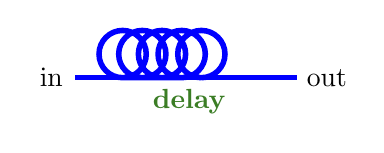
\begin{tikzpicture}
\node[minimum size=.6cm] (i) {in};
\node[xshift=+3.5cm,minimum size=.6cm] (o) {out};
\draw [-,line width=2pt, blue] ([xshift=4em] i.center)+(-0.5cm,0) arc (270:360+270:0.3) -- ([xshift=4em] i.center)+(-0.25cm,0) arc (270:360+270:0.3) -- ([xshift=4em] i.center) arc (270:360+270:0.3) -- ([xshift=4em] i.center)+(.25cm,0) arc (270:360+270:0.3) -- ([xshift=4em] i.center)+(.5cm,0) arc (270:360+270:0.3);
\draw [-,line width=2pt, blue] (i) -- (o);
\node[minimum size=.6cm, yshift=-0.3cm, xshift=+1.75cm] {\textbf{{\color{OliveGreen}delay}}};
\end{tikzpicture}  \\
\hline
 
\hline
\includegraphics[width=5cm,trim={2cm 8cm 2cm 7.5cm},clip]{figures/axi2dac.pdf} &Tuneable voltage source. \newline{\color{BlueViolet} Controllable states/constants.}&
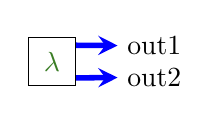
\begin{tikzpicture}
\node[draw, rectangle, minimum size=.6cm] (plus) {\textbf{{\color{OliveGreen}$\lambda$}}};
\node[xshift=+1.3cm, yshift=+0.2cm] (o) {out1};
\node[xshift=+1.3cm, yshift=-0.2cm] (o2) {out2};
\draw [->,>=stealth,line width=2pt,blue] ([yshift=-0.1cm] plus.north east) -- (o);
\draw [->,>=stealth,line width=2pt,blue] ([yshift=+0.1cm] plus.south east) -- (o2);
\end{tikzpicture}  \\

\hline
\includegraphics[width=5cm,trim={1cm 6.5cm 1cm 6cm},clip]{figures/nco.pdf} 
&\hspace*{0.8cm} DDS \newline {\color{BlueViolet}NCO}& 
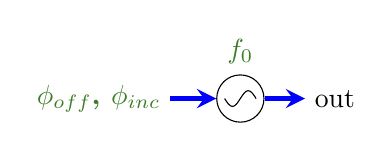
\begin{tikzpicture}	
\node [circle, draw ,minimum size=.6cm] (osc2){};
\node [minimum size=.6cm, yshift=+0.6cm] {\textbf{{\color{OliveGreen}$f_0$}}};
\draw ([xshift=-0.2cm] osc2.center) sin ([xshift=-0.10cm, yshift=-0.10cm] osc2.center) cos (osc2.center) sin ([xshift=0.10cm, yshift=0.10cm] osc2.center) cos ([xshift=0.2cm] osc2.center);
\node [xshift=-1.8cm] (l) {\textbf{{\color{OliveGreen}$\phi_{off}$, $\phi_{inc}$}}};
\node [xshift=+1.2cm] (r) {out};
\draw [->,>=stealth,line width=2pt,blue] (l) -- (osc2);
\draw [->,>=stealth,line width=2pt,blue] (osc2) -- (r);
\end{tikzpicture}  \\

\hline
\includegraphics[width=5cm,trim={1cm 6.5cm 1cm 6cm},clip]{figures/pid.pdf} &PID&
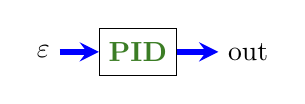
\begin{tikzpicture}
\node[draw, rectangle, minimum size=.6cm] (pid) {\textbf{{\color{OliveGreen}PID}}};
\node[xshift=-1.2cm] (i) {$\varepsilon$};
\node[xshift=+1.4cm] (o) {out};
\draw [->,>=stealth,line width=2pt,blue] (i) -- (pid);
\draw [->,>=stealth,line width=2pt,blue] (pid) -- (o);
\end{tikzpicture}   \\

\hline
\includegraphics[width=4.8cm,trim={1cm 7cm 1cm 6cm}, clip]{figures/dat2ram.pdf} &Monitoring: oscilloscope, spectrum analyzer...\newline {\color{BlueViolet}Can also be used to process the signal in the CPU. Up to 12 channels.} & 
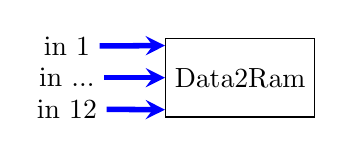
\begin{tikzpicture}
\node[draw, rectangle, minimum size=1cm] (dat) {Data2Ram};
\node[xshift=-2.2cm, yshift=+.4cm] (i1) {in 1};
\node[xshift=-2.2cm, yshift=-.4cm] (i2) {in 12};
\node[xshift=-2.2cm, yshift=0cm] (i) {in ...};
\draw [->,>=stealth,line width=2pt,blue] (i1) -- ([yshift=-.1cm] dat.north west);
\draw [->,>=stealth,line width=2pt,blue] (i2) -- ([yshift=+.1cm]dat.south west);
\draw [->,>=stealth,line width=2pt,blue] (i) -- (dat.west);
\end{tikzpicture}   \\

\hline
\end{tabular}

\section{Webserver}\label{sect:webserver}

The tuneable parameters of the IPs are controlled through C coded functions, visible in the /oscimpDigital/lib/my\_lib.h library files. Example of functions with a generic driver "fpgagen":

\vspace{-0.2cm}
\begin{lstlisting}[language=C]
fpgagen_send_conf(char *filename, int reg, int value); 
fpgagen_recv_conf(char *filename, int reg, int *value);
\end{lstlisting}

\hspace{1cm}

Those functions can be implemented in a graphic interface to constitute a user friendly control of the IPs. Here we show an example of webserver using RemI\footnote{Download and Faq : https://www.remigui.com/}, a cross platform remote gui for python. The wrapper liboscimp\_fpga.py makes the intermediary between the webserver and the libraries. It takes the following form:

\vspace{-0.2cm}
\begin{lstlisting}[language=Python]
import ctypes
from ctypes import *
lib = ctypes.CDLL('/usr/lib/liboscimp_fpga.so')

def fpgagen_send_conf(filename, reg, value):
		file = ctypes.create_string_buffer(str.encode(filename))
		my_val = int(value)
		lib.add_const_set_offset(file, reg, my_val)

def fpgagen_recv_conf(filename, reg):
		file = ctypes.create_string_buffer(str.encode(filename))
		my_val = c_int()
		ret_val = lib.fpgagen_recv_conf(file, reg, byref(my_val))
		return (ret_val, my_val.value)
\end{lstlisting}

\hspace{1cm}

Then the example of functions implemented in the webserver to configure the IPs is:

\vspace{-0.2cm}
\begin{lstlisting}[language=Python]
import liboscimp_fpga
liboscimp_fpga.fpgagen_send_conf("/dev/my_file", my_reg, my_value)
\end{lstlisting}

\hspace{1cm}

In the webserver, values sent to the IPs can either take the form of slider, a spinbox, a checkbox a button... In our case, a simple actuator will be represented by a checkbox, and any other controllable value by both a slider and a spinbox. The structure of the webserver ins as fallows:

\vspace{-0.2cm}
\begin{lstlisting}[language=Python]
#!/usr/bin/env python

import liboscimp_fpga
import ctypes
import remi.gui as gui
from remi import start, App

class MyApp(App):
		def __init__(self, *args):
				super(MyApp, self).__init__(*args)

		def main(self):
				self.w = gui.VBox()
				
				#Create the slider and the spinbox, whose value is restricted to -8192 to 8191 (no overflow)
				self.hbox_MY_VALUE = gui.HBox(margin="10px")
				self.lb_MY_VALUE = gui.Label("/dev/MY_VALUE_FILE", width="20%", margin="50px")
				self.sd_MY_VALUE = gui.Slider(0, -8192, 8191, 1, width="60%", margin="10px")
				self.sd_MY_VALUE.set_oninput_listener(self.sd_MY_VALUE_changed)
				self.sb_MY_VALUE = gui.SpinBox(0, -8192, 8191, 1, width="20%", margin="10px")
				self.sb_MY_VALUE.set_on_change_listener(self.sb_MY_VALUE_changed)
				self.sd_MY_VALUE_changed(self.sd_MY_VALUE, self.sd_MY_VALUE.get_value())
				self.hbox_MY_VALUE.append(self.lb_MY_VALUE)
				self.hbox_MY_VALUE.append(self.sd_MY_VALUE)
				self.hbox_MY_VALUE.append(self.sb_MY_VALUE)
				self.w.append(self.hbox_MY_VALUE)

				#Create the checkbox
				self.hbox_MY_ACTUATOR = gui.HBox(margin="10px")
				self.lb_MY_ACTUATOR = gui.Label("/dev/MY_ACTUATOR_FILE", width="20%", margin="50px")
				self.cb_MY_ACTUATOR = gui.CheckBox(True, width="5%", margin="10px")
				self.cb_MY_ACTUATOR.set_on_change_listener(self.cb_MY_ACTUATOR_changed)
				self.hbox_MY_ACTUATOR.append(self.lb_MY_ACTUATOR)
				self.hbox_MY_ACTUATOR.append(self.cb_MY_ACTUATOR)
				self.w.append(self.hbox_MY_ACTUATOR)

				return self.w
		
		#Function called by the slider
		def sd_MY_VALUE_changed(self, widget, value):
				print("/dev/MY_VALUE_FILE", MY_REG, int(value))
				liboscimp_fpga.fpgagen_send_conf("/dev/MY_VALUE_FILE", MY_REG, int(value))
				self.sb_MY_VALUE.set_value(int(value))

		#Function called by the spinbox
		def sb_MY_VALUE_changed(self, widget, value):
				print("/dev/MY_VALUE_FILE", MY_REG, int(value))
				liboscimp_fpga.fpgagen_send_conf("/dev/MY_VALUE_FILE", MY_REG, int(value))
				self.sd_MY_VALUE.set_value(int(float(value)))
				
		#Function called by the checkbox
		def sb_MY_ACTUATOR_changed(self, widget, value):
				print("/dev/MY_ACTUATOR_FILE", MY_REG, int(value))
				liboscimp_fpga.fpgagen_send_conf("/dev/MY_ACTUATOR_FILE", MY_REG2, int(value))
				self.sd_adc1_offset.set_value(int(float(value)))

#Launch oh the webserver on the local machine
start(MyApp, address="0.0.0.0", port=80, title="My_super_webserver")
\end{lstlisting}

Preview of the webserver created:

\begin{figure}[h!tb]
	\begin{center}
		\includegraphics[width=15cm]{webserver/Super_webserver.png}
		\caption{Example of webserver with MY\_VALUE\_FILE represented by a slider and a spinbox, and MY\_ACTUATOR\_FILE represented by a checkbox.}
		\label{fig:doubleDDS}
	\end{center}
\end{figure}

Here the generic driver fpgagen is used as an example, however the use of a different driver can lead to various requirements: arguments, data type, or several functions. Some specific cases will be treated in the next sections. In the other cases, refer to the /oscimpDigital/lib/my\_lib.h library files, or the oscimpDigital documentation: \href{[https://github.com/oscimp/oscimpDigital/tree/master/doc]}{https://github.com/oscimp/oscimpDigital/tree/master/doc}

\section{Double voltage source}

A double tuneable voltage source can be set up si using the axi\_to\_dac IP. However it's only one of the many functions that can be imagined with this IP. 
\newline See \href{[https://github.com/oscimp/oscimpDigital/blob/master/doc/IP/axi_to_dac.md]}{https://github.com/oscimp/oscimpDigital/blob/master/doc/IP/axi\_to\_dac.md}.
The block diagram is as follows :

\begin{figure}[h!tb]
	\begin{center}
		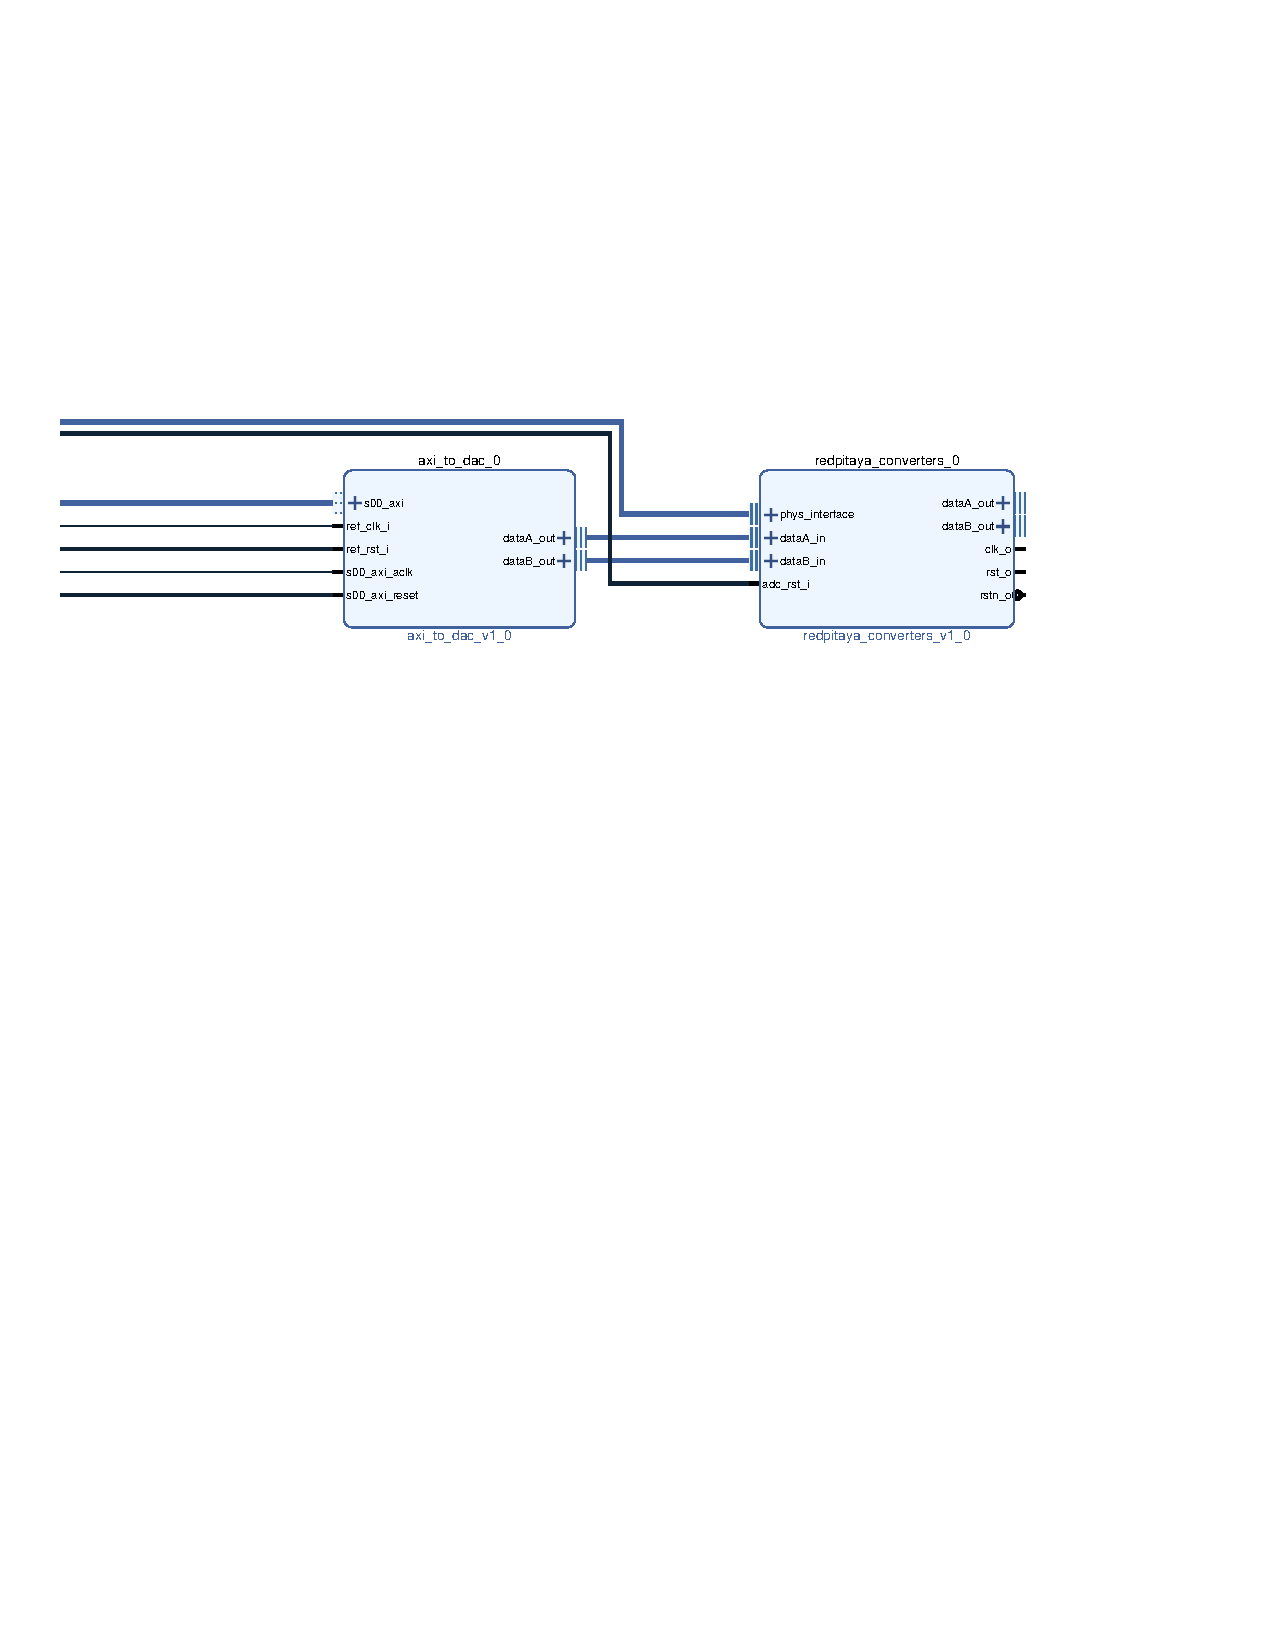
\includegraphics[width=10cm,trim={4.5cm 16cm 3.5cm 7cm}, clip]{figures/GeneTension.pdf}
		\caption{Part of the block diagram for the tuneable voltage source.}
		\label{fig:geneTension}
	\end{center}
\end{figure}

In this configuration and with data on $14~bits$, all the parameters of the axi\_to\_dac block keep their default value. The tuning of the output is performed with the webserver (see section \ref{sect:webserver}). With the Redpitaya board, the maximum voltage is $\pm 1~V$ per output.

\section{Double DDS}

The schematic configuration of the double DDS we propose here is shown below: 

\begin{center}
	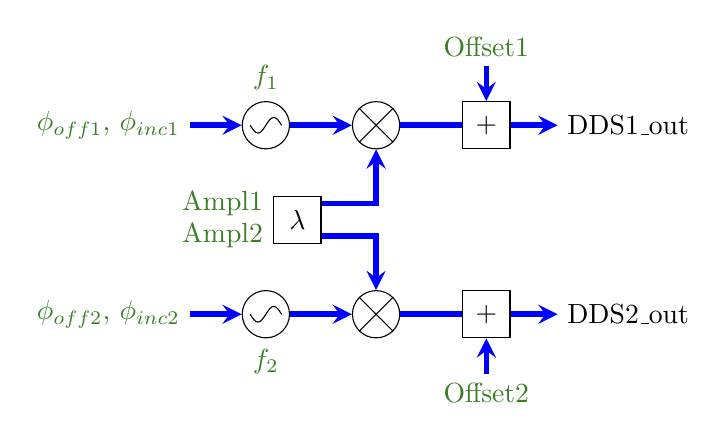
\begin{tikzpicture}	
\node[draw, rectangle, minimum size=.6cm] (plus) {$\lambda$};
\node[left of=plus, xshift=+0.05cm, yshift=+0.2cm] {{\color{OliveGreen}Ampl1}};
\node[left of=plus, xshift=+0.05cm, yshift=-0.2cm] {{\color{OliveGreen}Ampl2}};

\node [circle, draw ,minimum size=.6cm, xshift=-0.4cm, yshift=+0.2cm, above of=plus] (osc2){};
\node[above of=osc2, yshift=-0.4cm] {{\color{OliveGreen}$f_1$}};
\node [circle, draw ,minimum size=.6cm, xshift=-0.4cm, yshift=-0.2cm, below of=plus] (osc1){};
\node[below of=osc1, yshift=+0.4cm] {{\color{OliveGreen}$f_2$}};
\draw ([xshift=-0.2cm] osc2.center) sin ([xshift=-0.10cm, yshift=-0.10cm] osc2.center) cos (osc2.center) sin ([xshift=0.10cm, yshift=0.10cm] osc2.center) cos ([xshift=0.2cm] osc2.center);
\draw ([xshift=-0.2cm] osc1.center) sin ([xshift=-0.10cm, yshift=-0.10cm] osc1.center) cos (osc1.center) sin ([xshift=0.10cm, yshift=0.10cm] osc1.center) cos ([xshift=0.2cm] osc1.center);
\node [xshift=-1cm, left of=osc2] (l1) {{\color{OliveGreen}$\phi_{off1}$, $\phi_{inc1}$}};
\draw [->,>=stealth,line width=2pt,blue] (l1) -- (osc2);
\node [xshift=-1cm, left of=osc1] (l2) {{\color{OliveGreen}$\phi_{off2}$, $\phi_{inc2}$}};
\draw [->,>=stealth,line width=2pt,blue] (l2) -- (osc1);


\node [circle, draw ,minimum size=.6cm, xshift=0.4cm, right of= osc1] (mix1) {};
\draw [-] (mix1.south west) -- (mix1.north east);
\draw [-] (mix1.south east) -- (mix1.north west);
\node [circle, draw ,minimum size=.6cm, xshift=0.4cm, right of= osc2] (mix2) {};
\draw [-] (mix2.south west) -- (mix2.north east);
\draw [-] (mix2.south east) -- (mix2.north west);

\draw [->,>=stealth,line width=2pt,blue] ([yshift=-0.1cm] plus.north east) -| (mix2);
\draw [->,>=stealth,line width=2pt,blue] ([yshift=+0.1cm] plus.south east) -| (mix1);

\draw [->,>=stealth,line width=2pt,blue] (osc1) -- (mix1);
\draw [->,>=stealth,line width=2pt,blue] (osc2) -- (mix2);

\node[draw, rectangle, minimum size=.6cm, xshift=0.4cm, right of=mix1] (plu) {$+$};
\node[yshift=0cm, below of=plu] (c1) {{\color{OliveGreen}Offset2}};
\node[xshift=0.8cm, right of=plu] (o1) {DDS2\_out};
\draw [->,>=stealth,line width=2pt,blue] (plu) -- (o1);
\draw [->,>=stealth,line width=2pt,blue] (c1) -- (plu);

\node[draw, rectangle, minimum size=.6cm, xshift=0.4cm, right of=mix2] (plu2) {$+$};
\node[yshift=0cm, above of=plu2] (c2) {{\color{OliveGreen}Offset1}};
\node[xshift=0.8cm, right of=plu2] (o2) {DDS1\_out};
\draw [->,>=stealth,line width=2pt,blue] (plu2) -- (o2);
\draw [->,>=stealth,line width=2pt,blue] (c2) -- (plu2);

\draw [-,>=stealth,line width=2pt,blue] (mix1) -- (plu);
\draw [-,>=stealth,line width=2pt,blue] (mix2) -- (plu2);
\end{tikzpicture} 
\end{center} 

It corresponds to two DDS with adjustable frequency, amplitude, output offset, and referenced on the same clock. Frequency/phase and amplitude modulation are not represented here, but can be added using sections \ref{sect:AM} and \ref{sect:FM}. The block diagram associated with this scheme is as follows:

\begin{figure}[h!tb]
	\begin{center}
		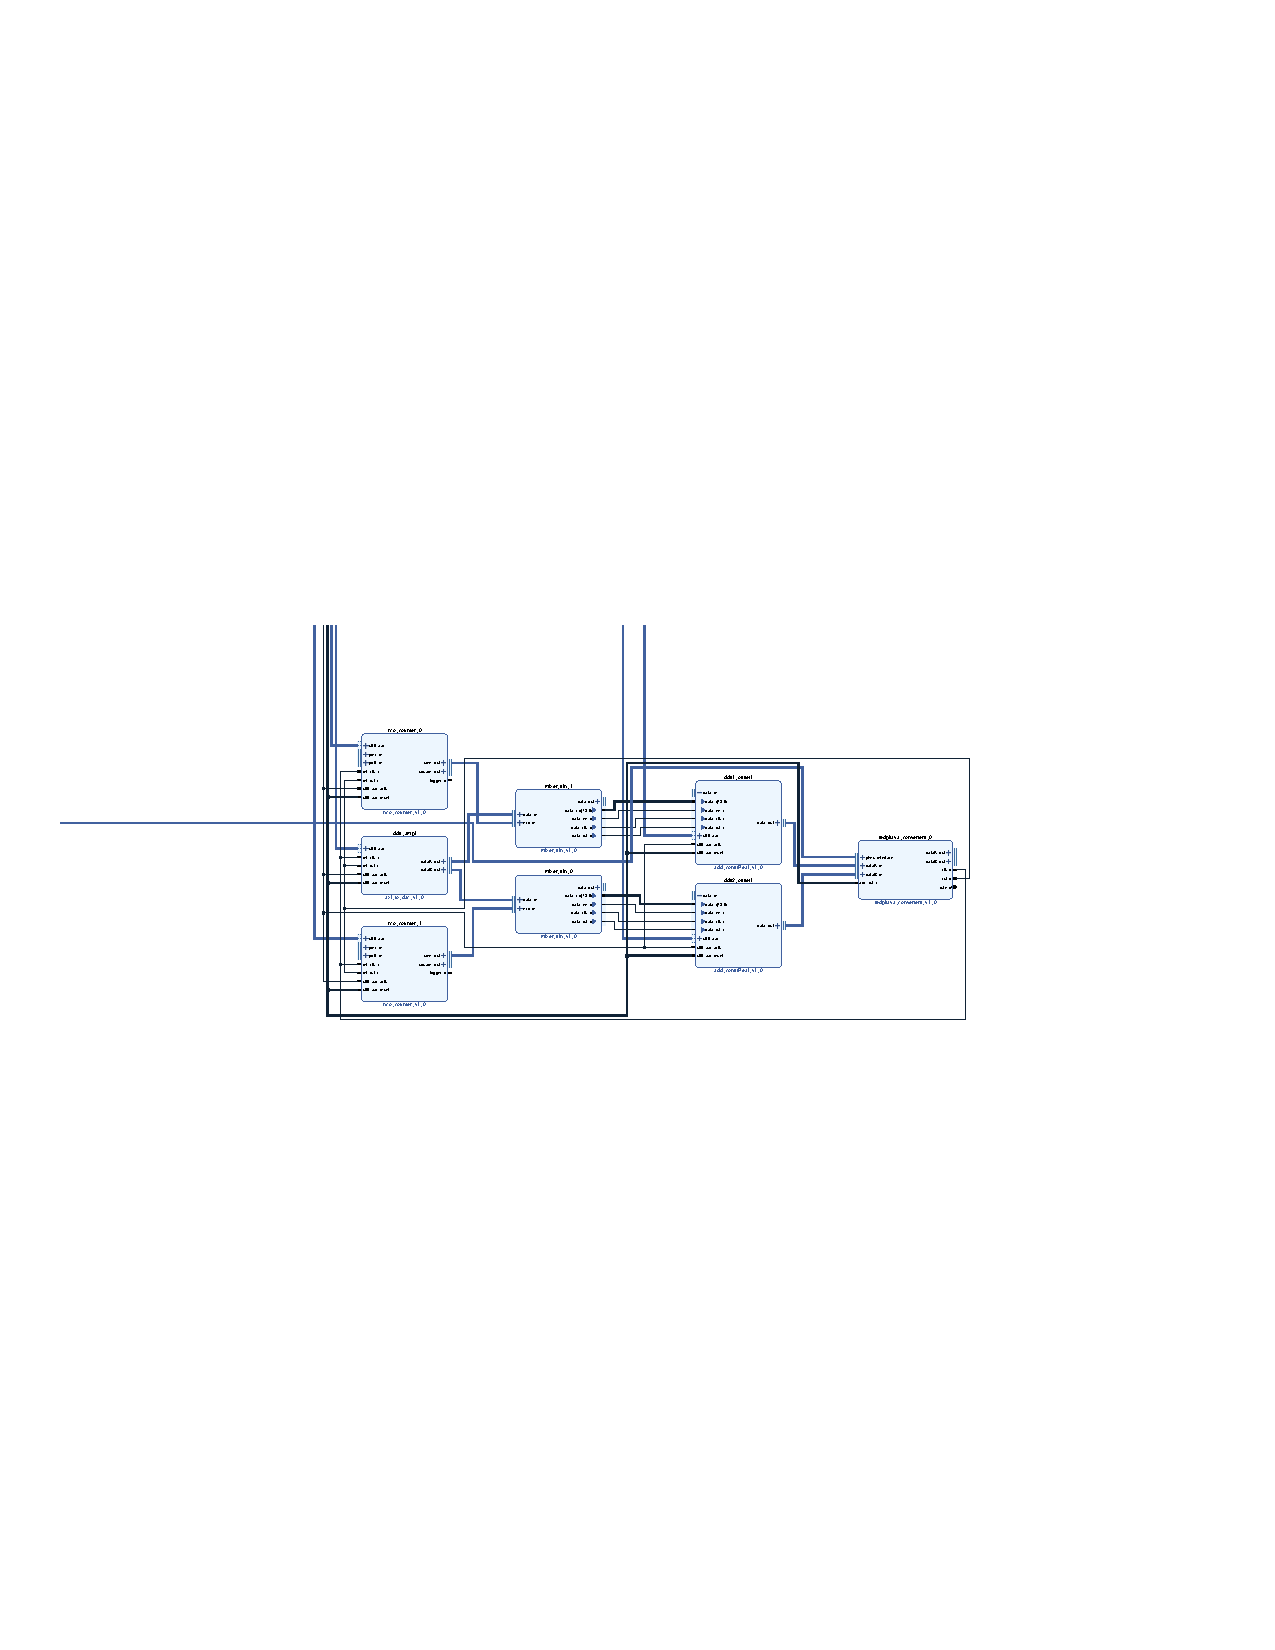
\includegraphics[width=16cm,trim={5cm 10.5cm 5cm 12cm}, clip]{figures/doubleDDS.pdf}
		\caption{Part of the block diagram for the double DDS.}
		\label{fig:doubleDDS}
	\end{center}
\end{figure}

\subsection{IP configuration}
\vspace{0.5cm}
The IPs configuration may change depending on the board/application, however in this example we used the following configurations:
\begin{center}
	\begin{tabular}{|>{\centering\arraybackslash}m{.3\linewidth} | >{\centering\arraybackslash}m{.3\linewidth} |}
\hline
IP & Configuration \\
\hline
 & Counter size: $40~bits$\\ nco\_counter &Data size: $16~bits$\\ &Lut size: $12~bits$ \\
\hline
axi\_to\_dac&Data size: $14~bits$ \\
\hline
mixer\_sin&Data size: $14~bits$ \newline Nco\_size: $16~bits$ \\
\hline
add\_constReal&Data in size: $14~bits$\newline Data out size: $14~bits$\newline Signed \\
\hline
\end{tabular}
\end{center}
\vspace{0.1cm}
\subsection{Webserver configuration}\label{subsec:doubleDDSws}

For the DDS offsets and amplitudes blocks we only use one value to be controlled, ie. one slider/spinbox. However the NCO block offers several options as the phase offset and increment can be internal or external to the block. Therefore we keep a default construction for the NCO in the webserver, including all these possibilities: 
\begin{itemize}
	\setlength\itemsep{-0.1cm}
	\item 1$^{st}$ slider+spinbox: the frequency control, up to the half clock frequency (Hz)
	\item 2$^{nd}$ slider+spinbox: the phase offset control
	\item pinc checkbox: internal or external phase increment
	\item poff checkbox: internal or external phase increment
\end{itemize} 

In the present case there is no external connections for the frequency and phase increments, thus the pinc and poff checkbox will remain checked. A preview of the webserver for the double DDS design is given in fig.\ref{fig:doubleDDS}.\newpage

\begin{figure}[!h!tb]
	\begin{center}
		\includegraphics[width=14cm]{webserver/2019-10-14-143651_927x541_scrot.png}
		\caption{Screenshot of the double DDS webserver.}
		\label{fig:doubleDDS}
	\end{center}
\end{figure}

\vspace{-1cm}

\subsection{Expected output}

We show in fig.\ref{fig:doubleDDSok} an example of twe signals generated. \newline 
Ch1: $f_0=30~MHz$, $dds1\_ampl=8191~samples$, $dds1\_offset=0~sample$, \newline $\phi_{off1}=0~sample$.\newline
Ch2: $f_0=45~MHz$, $dds2\_ampl=3000~samples$, $dds2\_offset=5000~samples$, \newline $\phi_{off2}=0~sample$.

\begin{figure}[h!tb]
	\begin{center}
		\includegraphics[width=14cm]{scope/doubleDDSok.pdf}
		\caption{Expected output.}
		\label{fig:doubleDDSok}
	\end{center}
\end{figure}

With an internal phase increment, the output signals are generated with an arbitrary phase. This phase can be adjusted according to the intended application, using the phase offset slider, as represented in fig.\ref{fig:doubleDDSphase}:

\begin{figure}[h!tb]
	\begin{center}
		\includegraphics[width=14cm]{scope/doubleDDSokPhi.pdf}
		\caption{Phase offset.}
		\label{fig:doubleDDSphase}
	\end{center}
\end{figure}

\vspace{-1cm}
\subsection{Unexpected output}\label{subsect:doubleDDSpasOk}

In fig.\ref{fig:doubleDDSpasOk} the Ch1 signal is the same, but there is an overflow in Ch2 due to the sum of $dds1\_ampl$ and $dds1\_offset$. \newline
Ch2: $f_0=45~MHz$, $dds2\_ampl=8191~samples$, $dds2\_offset=8191~samples$, \newline $\phi_{off2}=0~sample$.

\begin{figure}[!h!tb]
	\begin{center}
		\includegraphics[width=14cm]{scope/doubleDDSpasOk.pdf}
		\caption{Unexpexcted output due to overflow in ch2.}
		\label{fig:doubleDDSpasOk}
	\end{center}
\end{figure}
Solution: decrease either $dds1\_ampl$ or $dds1\_offset$, such as ${dds1\_ampl + dds1\_offset < 8191}$.

\section{Amplitude modulation V1}\label{sect:AM1}

An amplitude modulation can be performed easily, in the same way as with RF components:

\begin{center}
	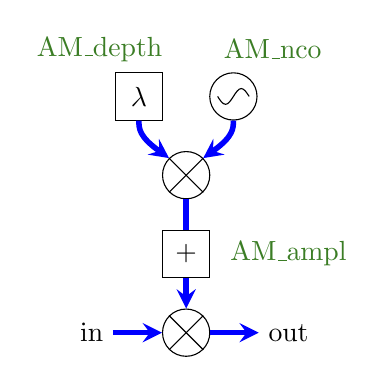
\begin{tikzpicture}	
	\node[draw, rectangle, minimum size=.6cm] (plus) {$\lambda$};
	\node[above of=plus, yshift=-0.4cm, xshift=-0.5cm] {{\color{OliveGreen}AM\_depth}};
	\node [circle, draw ,minimum size=.6cm, xshift=+0.6cm, below of=plus] (mix1) {};
	\draw [-] (mix1.south west) -- (mix1.north east);
	\draw [-] (mix1.south east) -- (mix1.north west);
	\node[draw, rectangle, minimum size=.6cm, below of=mix1] (plu) {+};
	\node[right of=plu, xshift=+0.3cm] {{\color{OliveGreen}AM\_ampl}};
	\node [circle, draw ,minimum size=.6cm, below of=plu] (mix2) {};
	\draw [-] (mix2.south west) -- (mix2.north east);
	\draw [-] (mix2.south east) -- (mix2.north west);
	
	\node [circle, draw ,minimum size=.6cm, above of=mix1, xshift=0.6cm] (osc1){};
	\node[above of=osc1, yshift=-0.4cm, xshift=+0.5cm] {{\color{OliveGreen}AM\_nco}};
	\draw ([xshift=-0.2cm] osc1.center) sin ([xshift=-0.10cm, yshift=-0.10cm] osc1.center) cos (osc1.center) sin ([xshift=0.10cm, yshift=0.10cm] osc1.center) cos ([xshift=0.2cm] osc1.center);
	
	\node[xshift=0.8cm, left of=mix2, xshift=-1cm] (i1) {in};
	\node[xshift=0.8cm, right of=mix2, xshift=-0.5cm] (o1) {out};
	\draw [->,>=stealth,line width=2pt,blue] (mix2) -- (o1);
	\draw [->,>=stealth,line width=2pt,blue] (i1) -- (mix2);
	\draw [->,>=stealth,line width=2pt,blue] (plu) -- (mix2);
	\draw [-,line width=2pt,blue] (mix1) -- (plu);
	
	\draw [->, >=stealth, line width=2pt, blue] (plus.south) .. controls ([xshift=0cm, yshift=-0.1cm] plus.south) and ([xshift=0em, yshift=-0.2cm] plus.south) ..(mix1.north west);
	
	\draw [->, >=stealth, line width=2pt, blue] (osc1.south) .. controls ([xshift=0cm, yshift=-0.1cm] osc1.south) and ([xshift=0em, yshift=-0.2cm] osc1.south) ..(mix1.north east);
	\end{tikzpicture} 
\end{center}

This scheme is equivalent to the expression of the amplitude modulation:
\begin{center}
	 ${y(t)=[1 + h~cos(\omega_m t)]z(t)}$\newline
	
	 $\Rightarrow{out=[1 + \frac{AM\_depth}{AM\_ampl} AM\_nco]~AM\_ampl\times in}$
\end{center}

Then the modulation depth is $h=\frac{AM\_depth}{AM\_ampl}$. Thereafter:

\begin{itemize}
	\setlength\itemsep{-0.1cm}
	\item $h=0$ with $AM\_depth=0$ 
	\item $h=0.5$ with $AM\_depth=4096~samples$ and $AM\_ampl=8191~samples$
	\item $h=1$ with $AM\_depth=8191~samples$ and $AM\_ampl=8191~samples$
	\item $h=2$ with $AM\_depth=8191~samples$ and $AM\_ampl=4096~samples$
\end{itemize}

The block diagram corresponding to this scheme is as follows:

\begin{figure}[h!tb]
	\begin{center}
		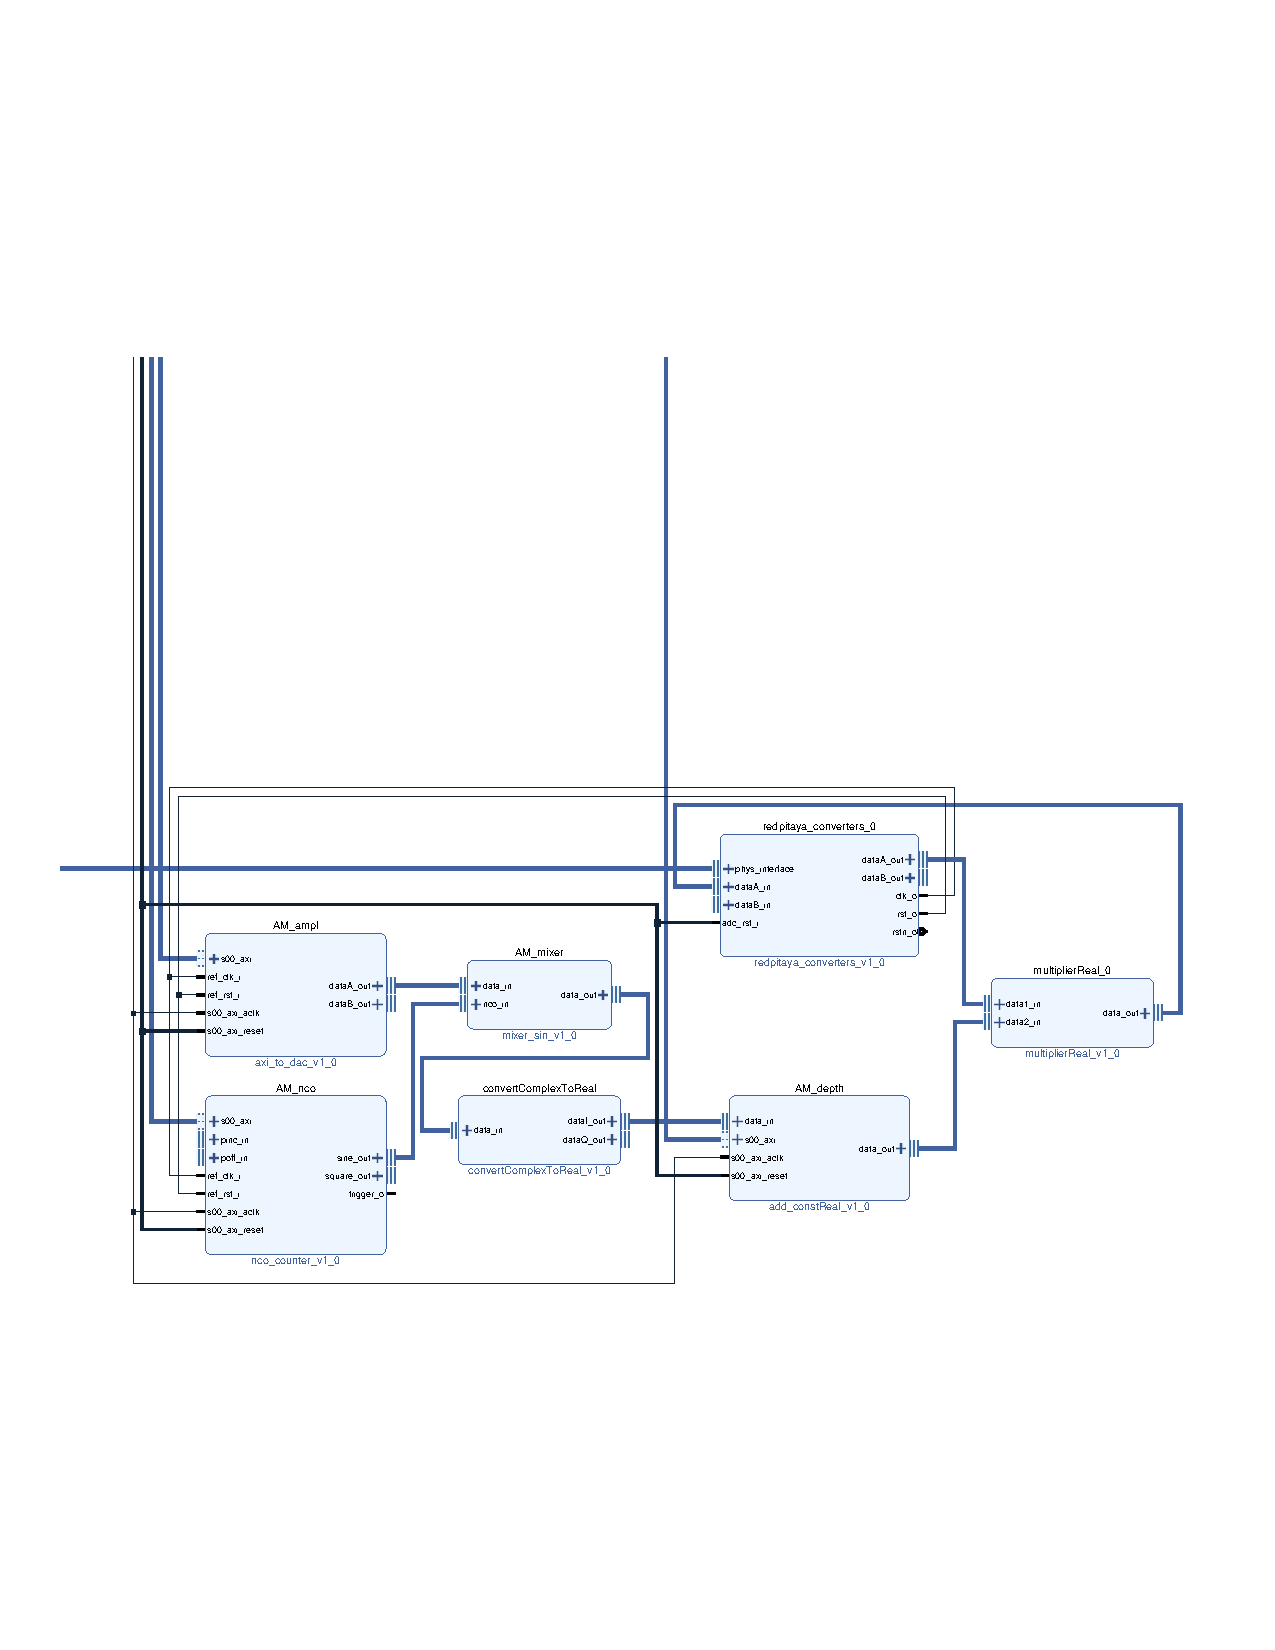
\includegraphics[width=15cm,trim={2cm 5cm 2cm 14cm}, clip]{design/mod_ampl1.pdf}
		\caption{Part of the block diagram for this amplitude modulation.}
		\label{fig:mod_ampl1}
	\end{center}
\end{figure}

In this block diagram the input and output are connected to the converters block to make an example with external signal. However this principle can be included to other applications, such as the double dds design to add an amplitude modulation option to the generated signals.

\subsection{IP configuration}
\vspace{0.5cm}
IPs configuration in this example:
\begin{center}
	\begin{tabular}{|>{\centering\arraybackslash}m{.3\linewidth} | >{\centering\arraybackslash}m{.3\linewidth} |}
		\hline
		IP & Configuration \\
		\hline
		& Counter size: $40~bits$\\ nco\_counter &Data size: $16~bits$\\ &Lut size: $12~bits$ \\
		\hline
		axi\_to\_dac&Data size: $16~bits$ \\
		\hline
		mixer\_sin\_1&Data size: $16~bits$ \newline Nco\_size: $16~bits$ \\
		mixer\_sin\_2&Data size: $14~bits$ \newline Nco\_size: $16~bits$ \\
		\hline
		& Data in size: $16~bits$\\add\_const\_real & Data out size: $14~bits$\\ &Format: Signed \\
		\hline
	\end{tabular}
\end{center}
\vspace{0.1cm}
\subsection{Webserver configuration}

Here the webserver configuration is similar to the double dds one. In case refer to subsection \ref{subsec:doubleDDSws}. preview of the amplitude modulation part of the webserver, with the mod\_nco controlling the modulation frequency, and mod\_ampl controlling it's amplitude:

\begin{figure}[!h!tb]
	\begin{center}
		\includegraphics[width=14cm]{webserver/AM_V1.png}
		\caption{Screenshot of the amplitude modulation part of the webserver.}
		\label{fig:amplModWsv1}
	\end{center}
\end{figure}
\vspace{-1cm}

\subsection{Expected output}

To make a small preview of the expected behavior of the amplitude modulation, first we set the $AM\_ampl$ to $8191~samples$  we use at the input a sine signal of $5~MHz$ and $0~dBm$.
With an amplitude modulation of $50~MHz$ and $1000~samples$, we expect: \newpage

\subsection{Unexpected output}

\section{Amplitude modulation V2}\label{sect:AM2}

Another way to modulate the amplitude is presented here. Although it does not correspond to the known definition of an amplitude modulation, it can be useful to perform a scan acting on the amplitude of a given signal. An example is performing a frequency scan with a laser diode, by acting on its current control. The scheme used is quite similar:

\begin{center}
	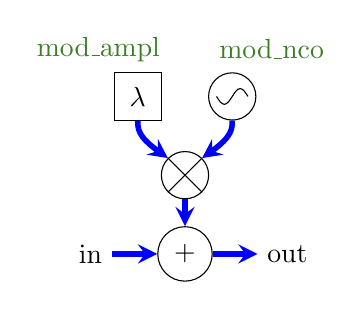
\begin{tikzpicture}	
	\node[draw, rectangle, minimum size=.6cm] (plus) {$\lambda$};
	\node[above of=plus, yshift=-0.4cm, xshift=-0.5cm] {{\color{OliveGreen}mod\_ampl}};
	\node [circle, draw ,minimum size=.6cm, xshift=+0.6cm, below of=plus] (mix1) {};
	\draw [-] (mix1.south west) -- (mix1.north east);
	\draw [-] (mix1.south east) -- (mix1.north west);
	\node [circle, draw ,minimum size=.6cm, below of=mix1] (mix2) {+};
	
	\node [circle, draw ,minimum size=.6cm, above of=mix1, xshift=0.6cm] (osc1){};
	\node[above of=osc1, yshift=-0.4cm, xshift=+0.5cm] {{\color{OliveGreen}mod\_nco}};
	\draw ([xshift=-0.2cm] osc1.center) sin ([xshift=-0.10cm, yshift=-0.10cm] osc1.center) cos (osc1.center) sin ([xshift=0.10cm, yshift=0.10cm] osc1.center) cos ([xshift=0.2cm] osc1.center);
	
	\node[xshift=0.8cm, left of=mix2, xshift=-1cm] (i1) {in};
	\node[xshift=0.8cm, right of=mix2, xshift=-0.5cm] (o1) {out};
	\draw [->,>=stealth,line width=2pt,blue] (mix2) -- (o1);
	\draw [->,>=stealth,line width=2pt,blue] (i1) -- (mix2);
	\draw [->,>=stealth,line width=2pt,blue] (mix1) -- (mix2);
	
	\draw [->, >=stealth, line width=2pt, blue] (plus.south) .. controls ([xshift=0cm, yshift=-0.1cm] plus.south) and ([xshift=0em, yshift=-0.2cm] plus.south) ..(mix1.north west);
	
	\draw [->, >=stealth, line width=2pt, blue] (osc1.south) .. controls ([xshift=0cm, yshift=-0.1cm] osc1.south) and ([xshift=0em, yshift=-0.2cm] osc1.south) ..(mix1.north east);
	\end{tikzpicture} 
\end{center}

The block diagram corresponding to this scheme is as follows:

\begin{figure}[h!tb]
	\begin{center}
		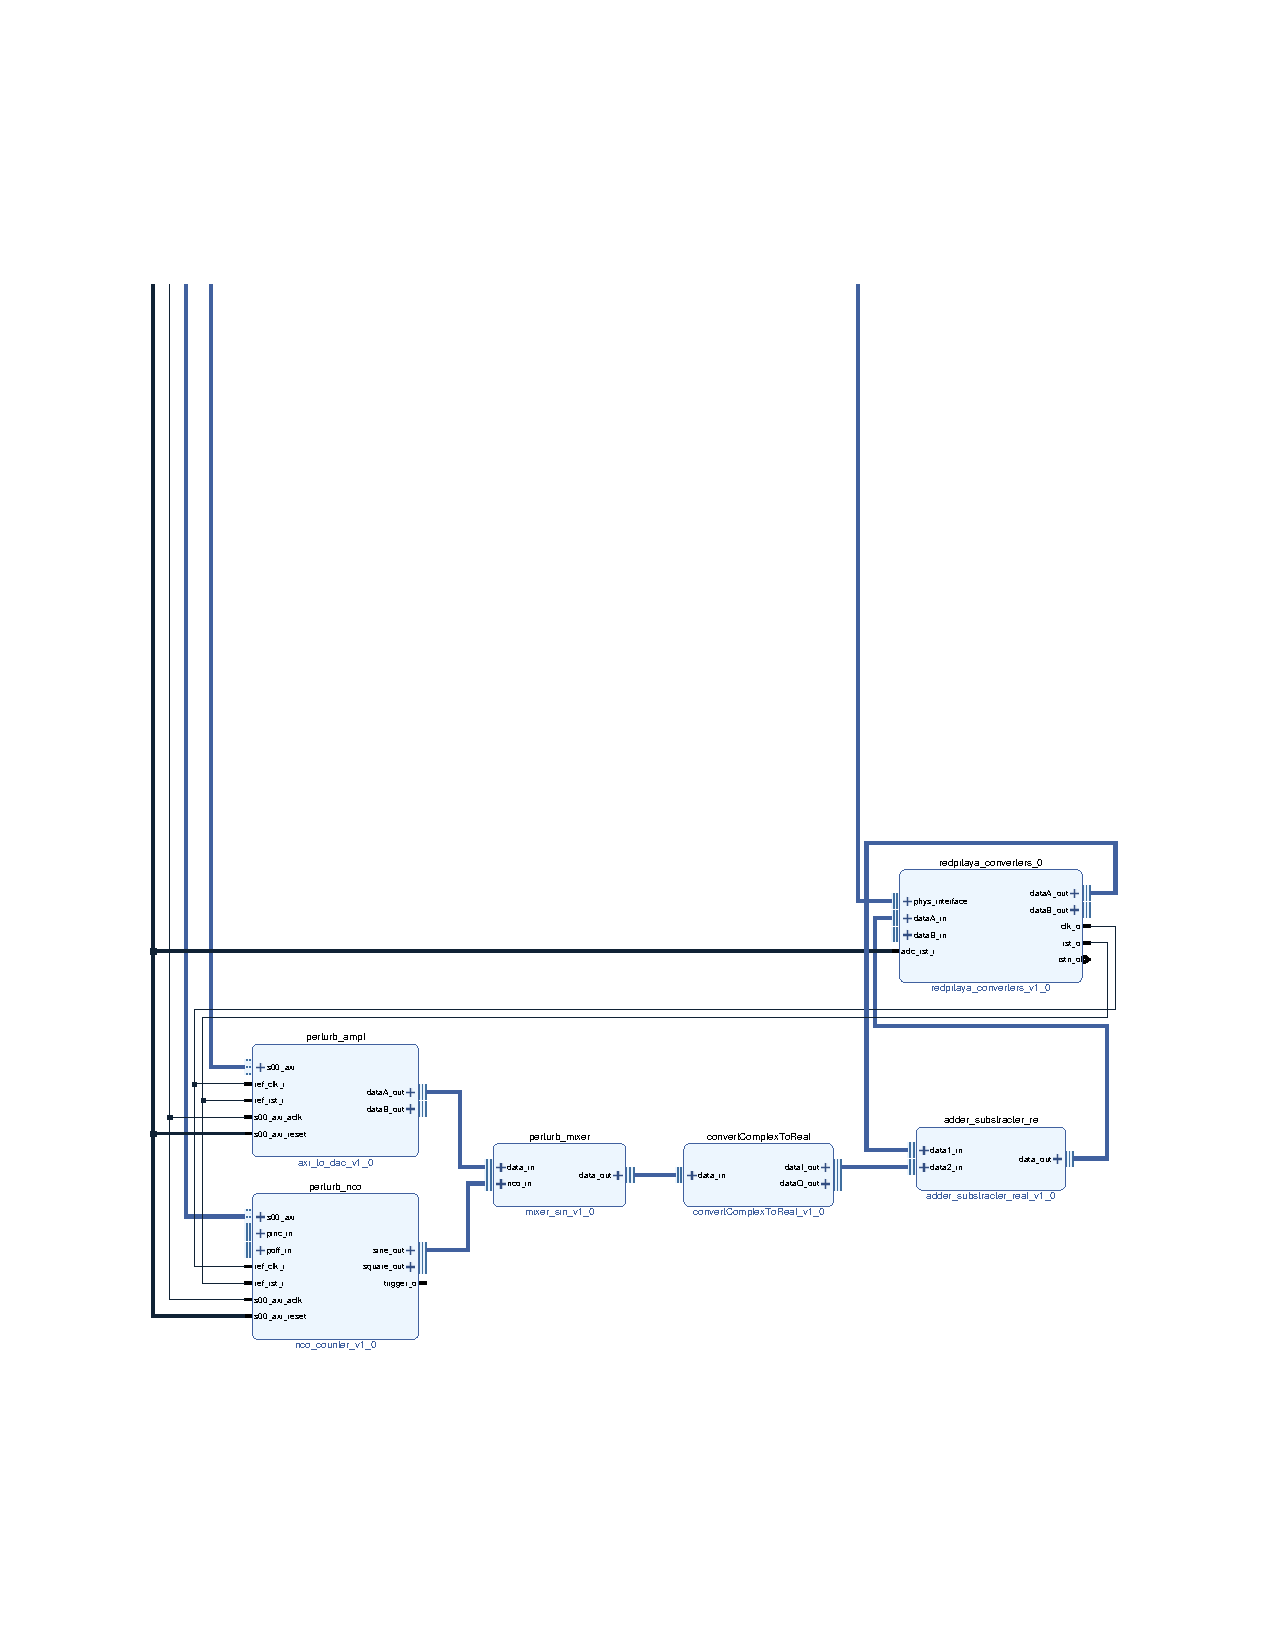
\includegraphics[width=16cm,trim={3cm 6cm 4cm 13cm}, clip]{design/mod_ampl.pdf}
		\caption{Part of the block diagram for the amplitude modulation.}
		\label{fig:mod_ampl}
	\end{center}
\end{figure}


\subsection{IP configuration}
\vspace{0.5cm}
IPs configuration in this example:
\begin{center}
	\begin{tabular}{|>{\centering\arraybackslash}m{.3\linewidth} | >{\centering\arraybackslash}m{.3\linewidth} |}
		\hline
		IP & Configuration \\
		\hline
		& Counter size: $40~bits$\\ nco\_counter &Data size: $16~bits$\\ &Lut size: $12~bits$ \\
		\hline
		axi\_to\_dac&Data size: $14~bits$ \\
		\hline
		mixer\_sin&Data size: $14~bits$ \newline Nco\_size: $16~bits$ \\
		\hline
		& Data size: $14~bits$\\adder\_substracter\_real & Operation: add\\ &Format: Signed \\
		\hline
	\end{tabular}
\end{center}
\vspace{0.1cm}
\subsection{Webserver configuration}


\begin{figure}[!h!tb]
	\begin{center}
		\includegraphics[width=14cm]{figures/ampl_mod_webserver.png}
		\caption{Screenshot of the amplitude modulation part of the webserver.}
		\label{fig:amplModWs}
	\end{center}
\end{figure}
\vspace{-1cm}

\subsection{Expected output}
We use at the input a sine signal of $5~MHz$ and $0~dBm$.
With an amplitude modulation of $50~MHz$ and $1000~samples$, we expect: \newpage

\begin{figure}[!h!tb]
	\begin{center}
		\includegraphics[width=14cm]{scope/Mod_amplOk.pdf}
		\caption{Expected behavior with input sine at $5~MHz$ and amplitude modulation of $50~MHz$.}
		\label{fig:ampleModOK}
	\end{center}
\end{figure}

\subsection{Unexpected output}

An unexpected situation can be the output signal visible in figure \ref{fig:ampleModPasOK}: 

\begin{figure}[!h!tb]
	\begin{center}
		\includegraphics[width=14cm]{scope/Mod_amplPasOk.pdf}
		\caption{Unexpected behavior with input sine at $5~MHz$ and amplitude modulation of $50~MHz$.}
		\label{fig:ampleModPasOK}
	\end{center}
\end{figure}

This situation is very similar to the fig.\ref{fig:doubleDDSpasOk} in subsection \ref{subsect:doubleDDSpasOk}: this output is a result of an overflow happening during the signal processing. This situation is due to an input signal too powerful with respect to the modulation depth.
Solution: decrease the modulation depth or the power of the input signal. 


\section{Frequency and phase modulation of a NCO}\label{sect:FMPM}

\begin{center}
	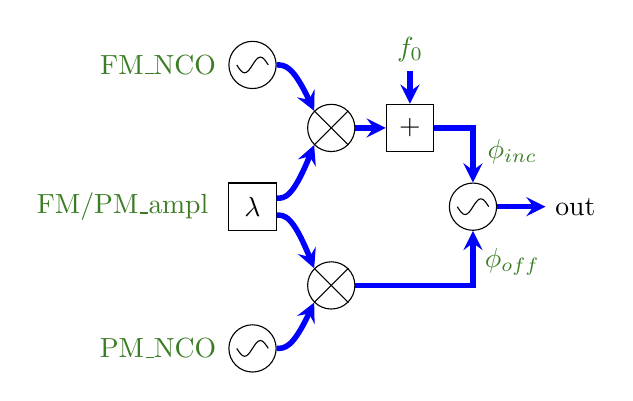
\begin{tikzpicture}	
\node [circle, draw ,minimum size=.6cm] (osc1){};
\draw ([xshift=-0.2cm] osc1.center) sin ([xshift=-0.10cm, yshift=-0.10cm] osc1.center) cos (osc1.center) sin ([xshift=0.10cm, yshift=0.10cm] osc1.center) cos ([xshift=0.2cm] osc1.center);

\node[xshift=0.8cm, right of=osc1, xshift=-0.5cm] (o1) {out};
\draw [->,>=stealth,line width=2pt,blue] (osc1) -- (o1);

\node[draw, rectangle, minimum size=.6cm, left of=osc1, xshift=0.2cm, above of=osc1] (plus) {$+$};
\draw [->,>=stealth,line width=2pt,blue] (plus.east) -| (osc1.north);

\node [circle, draw ,minimum size=.6cm, left of=plus] (mix1) {};
\draw [-] (mix1.south west) -- (mix1.north east);
\draw [-] (mix1.south east) -- (mix1.north west);
\node [circle, draw ,minimum size=.6cm, xshift=0.2cm, left of=plus, left of=plus, below of=osc1] (mix2) {};
\draw [-] (mix2.south west) -- (mix2.north east);
\draw [-] (mix2.south east) -- (mix2.north west);
\node[above of=plus] (f0) {{\color{OliveGreen}$f_0$}};
\draw [->,>=stealth,line width=2pt,blue] (f0) -- (plus);

\draw [->,>=stealth,line width=2pt,blue] (mix1) -- (plus);
\draw [->,>=stealth,line width=2pt,blue] (mix2) -| (osc1.south);

\node [circle, draw ,minimum size=.6cm, above of=mix1, left of=mix1, yshift=-0.2cm] (osc2){};
\draw ([xshift=-0.2cm] osc2.center) sin ([xshift=-0.10cm, yshift=-0.10cm] osc2.center) cos (osc2.center) sin ([xshift=0.10cm, yshift=0.10cm] osc2.center) cos ([xshift=0.2cm] osc2.center);

\node [circle, draw ,minimum size=.6cm, below of=mix2, left of=mix2, yshift=0.2cm] (osc3){};
\draw ([xshift=-0.2cm] osc3.center) sin ([xshift=-0.10cm, yshift=-0.10cm] osc3.center) cos (osc3.center) sin ([xshift=0.10cm, yshift=0.10cm] osc3.center) cos ([xshift=0.2cm] osc3.center);

\node[draw, rectangle, minimum size=.6cm, left of=osc1, xshift=-1.8cm] (mampl) {$\lambda$};

\draw [->, >=stealth, line width=2pt, blue] (osc2.east) .. controls ([xshift=0.1cm, yshift=0cm] osc2.east) and ([xshift=0.2cm, yshift=0cm] osc2.east) ..(mix1.north west);
\draw [->, >=stealth, line width=2pt, blue] (osc3.east) .. controls ([xshift=0.1cm, yshift=0cm] osc3.east) and ([xshift=0.2cm, yshift=0cm] osc3.east) ..(mix2.south west);

\draw [->, >=stealth, line width=2pt, blue] ([yshift=0.2cm] mampl.south east) .. controls ([xshift=0.1cm, yshift=0.2cm] mampl.south east) and ([xshift=0.2cm, yshift=0.2cm] mampl.south east) ..(mix2.north west);

\draw [->, >=stealth, line width=2pt, blue] ([yshift=-0.2cm] mampl.north east) .. controls ([xshift=0.1cm, yshift=-0.2cm] mampl.north east) and ([xshift=0.2cm, yshift=-0.2cm] mampl.north east) ..(mix1.south west);

\node[left of=osc2, xshift=-0.2cm] () {{\color{OliveGreen}FM\_NCO}};
\node[left of=osc3, xshift=-0.2cm] () {{\color{OliveGreen}PM\_NCO}};
\node[left of=mampl, xshift=-0.65cm] () {{\color{OliveGreen}FM/PM\_ampl}};
\node[xshift=+0.5cm, yshift=+0.7cm] () {{\color{OliveGreen}$\phi_{inc}$}};
\node[xshift=+0.5cm, yshift=-0.7cm] () {{\color{OliveGreen}$\phi_{off}$}};
\end{tikzpicture} \\
\end{center}


\begin{figure}[h!tb]
	\begin{center}
		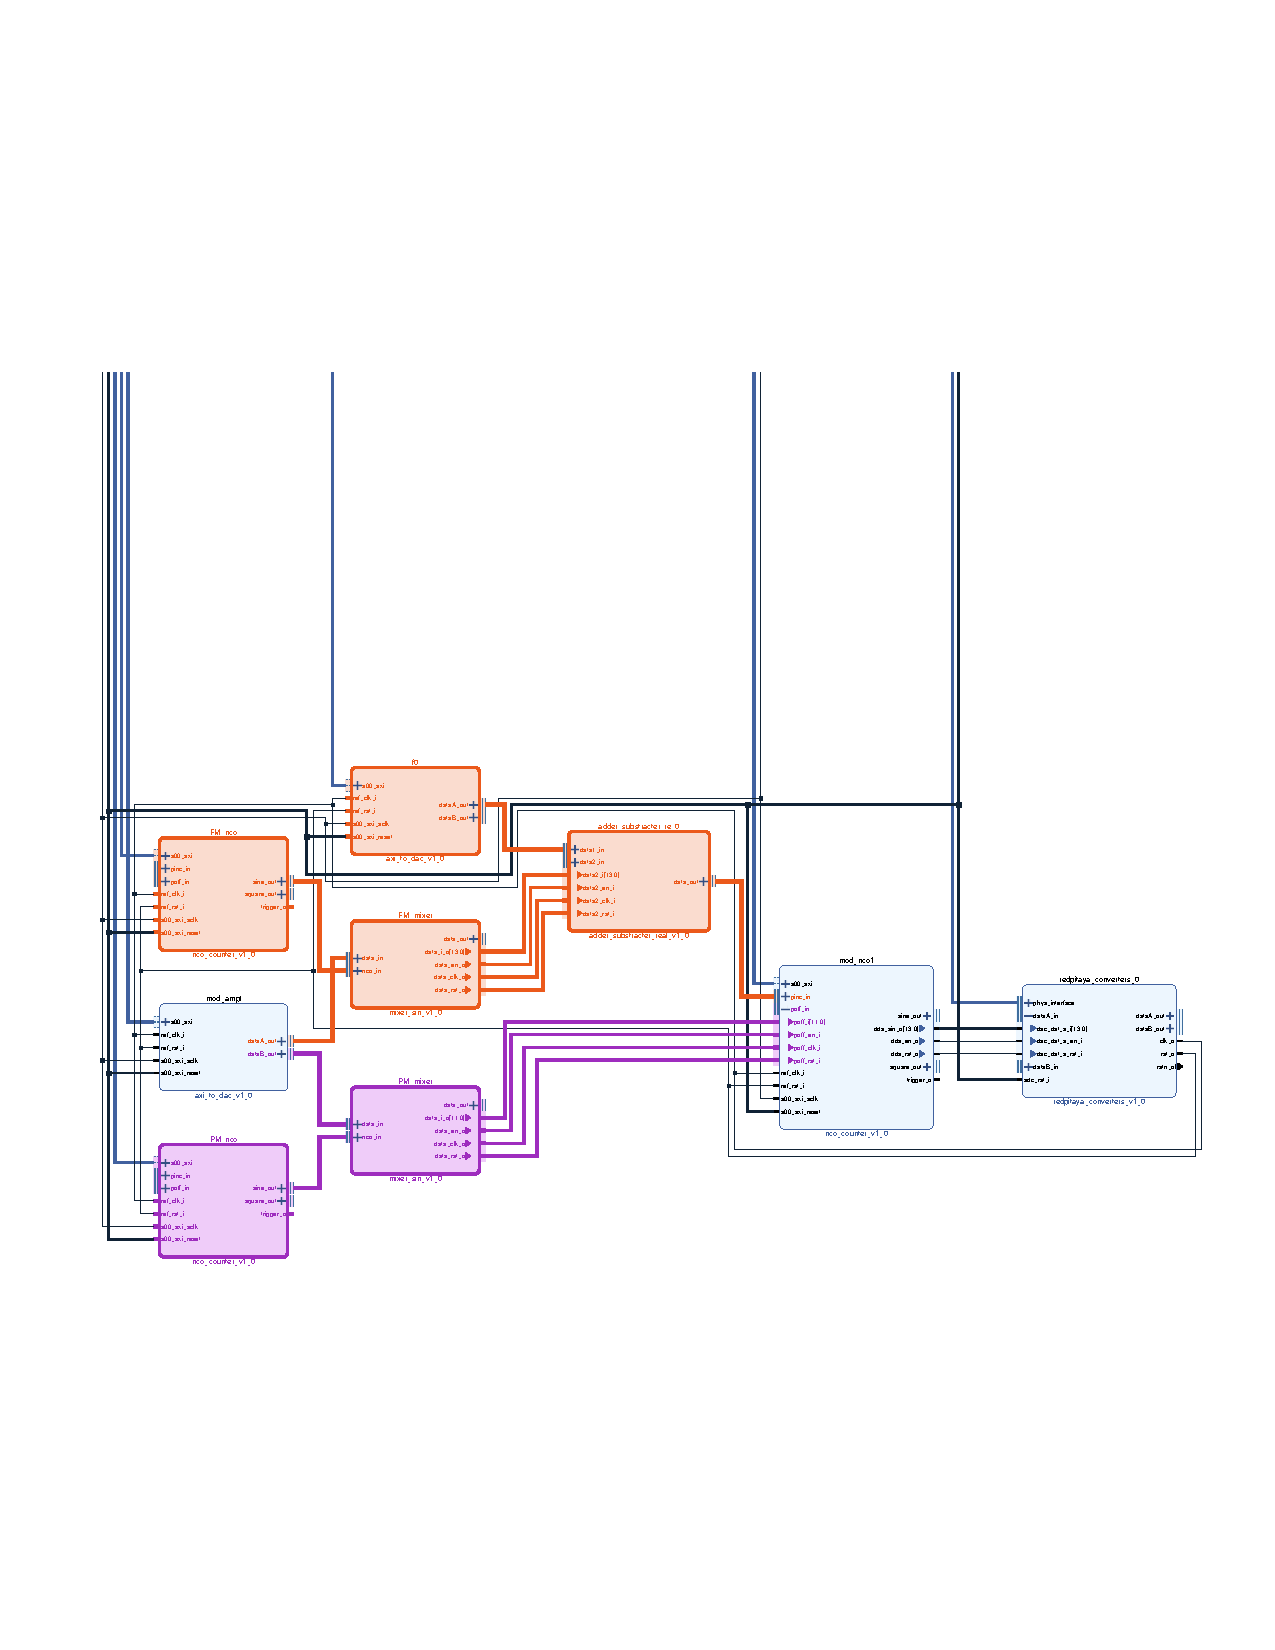
\includegraphics[width=16cm,trim={1.5cm 6.5cm 1cm 12.5cm}, clip]{design/FMPM.pdf}
		\caption{Part of the block diagram for frequency (orange) and phase (purple) modulation of a NCO.}
		\label{fig:mod_ampl}
	\end{center}
\end{figure}


%\begin{verbatim}
%insert code verbatim xml
%\end{verbatim}

\end{document}

cp ./project_1.runs/impl_1/design_1_wrapper.bit .
bootgen -image design_1_wrapper.bif -arch zynq -process_bitstream bin

jmfriedt@rugged:~/xilinx/oimp/doc/tutorials/4-fpga_FIR/project_1/app$ /home/jmfriedt/enseignement/ufr/platforms/redpitaya/buildroot-2018.08.1/output/build/linux-3f3c7b60919d56119a68813998d3005bca501a40/scripts/dtc/dtc -@ -I dts -O dtb -o project_1.dtbo project_1.dts

 source /home/jmfriedt/xilinx/oimp/fpga_driver/sourceme.ggm 
 export BOARD_NAME=redpitaya
 export BR_DIR=/home/jmfriedt/enseignement/ufr/platforms/redpitaya/buildroot-2018.08.1/
 make


/home/jmfriedt/enseignement/ufr/platforms/redpitaya/buildroot-2018.08.1/output/host/usr/bin/arm-linux-gcc -I /home/jmfriedt/xilinx/oimp/fpga_lib -o ma_lecture ma_lecture.c -L/home/jmfriedt/xilinx/oimp/fpga_lib -loscimp_fpga
